\chapter{Vorgehensweise} 
Im folgenden Kapitel beschäftige ich mich mit der Ausarbeitung theoretischer Grundlagen als auch mit der groben Planung des Algorithmus und deren Komponenten.
\section{Überblick zum genetischen Algorithmus}
Genetische Algorithmen versuchen die Prozesse der natürlichen Evolution nachzuahmen. Dabei wird initial eine Population von möglichst unterschiedlichen Individuen erstellt, hier eine Konfiguration aus Hyperparameter, die dann durch die Fitness-Funktion bewertet wird. Ein niedriger Wert bei der Fitnessfunktion bedeutet eine gute Lösung. Mittels einer Selektion werden schlechtere Konfigurationen entfernt, sodass durch eine Kombination mehrerer guter Lösungen wieder bessere entstehen können. Um eine große Diversität zu gewährleisten, werden die einzelnen Individuen mutiert, dabei werden einzelne Merkmale arithmetisch verschoben. Dieser Prozess wiederholt sich ständig, sodass weitere, womöglich bessere, Konfiguration entdeckt werden.
\tikzstyle{block} = [rectangle, draw, text width=10em, text centered, rounded corners, minimum height=3em]
\begin{figure}[h]
	\centering
	\begin{tikzpicture}
		[node distance=1.8cm,
		start chain=going below,]
		\node (n1) at (0,0) [block]  {Selektion};
		\node (n2) [block, below of=n1] {Rekombination};
		\node (n3) [block, below of=n2] {Mutation};
		\node (n4) [block, below of=n3] {Berechnung Fitness};
		\node (n5) [block, left of=n4, node distance=2in] {Start:\\Population erzeugen};
		% Connectors
		\draw [->] (n1) -- (n2);
		\draw [->] (n2) -- (n3);
		\draw [->] (n3) -- (n4);
		\draw [->] (n5) -- (n4);
		\draw [->] (n4.east) -| ++(1,0) |- (n1.east);
	\end{tikzpicture}
	\caption{Grundschema Genetischer Algorithmus \parencite[Seite 5]{stelldinger_naturanaloge_2024}}
\end{figure}
\section{Überblick Neuronale Netze}
Neuronale Netze sind eine Form des überwachten Lernens, das heißt sie lernen anhand von bereits bekannten Zielwerten. Im Beispiel der Klassifikation von Tierbildern ist beim überwachten Lernen bereits für jedes Bild bekannt, um welches Tier es sich dabei handelt. Das neuronale Netz erkennt selbstständig Muster in den Tierbildern, welche dann zur Generalisierung unbekannter Daten verwendet werden. Ziel hierbei ist die Extraktion der wichtigen Merkmale, nicht das stupide Auswendiglernen der Daten (\textit{"Overfitting"}). Das neuronale Netz wird dabei mit Trainingsdaten gefüttert, anhand dessen die Muster gelernt werden. Üblicherweise wird die Effektivität oder Genauigkeit des Modells an Daten überprüft, die nicht zum Training gehören \parencite{sonnet_neuronale_2022}.
\subsection{Hyperparameter in neuronalen Netzen}
Hyperparameter sind Parameter, welche den Lernprozess betreffen. Im Kontrast zu den Modellparametern, die während des Trainings aufgebaut werden, sind Hyperparameter beim Training bereits bekannt. Es gibt viele neuronale Netze, die Erfolg mit dynamischen Parametern haben \parencite{schaul_no_2013}. Andere typische Hyperparameter eines neuronalen Netzes beinhalten die Batch-Größe, Anzahl von Epochen sowie auch die Anzahl von Neuronen in der verdeckten Schicht. In dieser Hausarbeit beschränke ich mich auf die genannten Parameter.
\section{Aufbau des Genetischen Algorithmus}
Im nachfolgenden Kapitel beschäftige ich mich mit der Planung des genetischen Algorithmus, dabei wird auf die einzelnen Operationen eingegangen.
\subsection{Chromosom}
Ein Chromosome wird üblicherweise in binärer Darstellung kodiert. Dies hat den Vorteil, dass bitweise Operationen sehr effizient und schnell umsetzbar sind. Allerdings kann dies auch zu Problemen führen. Bei der Mutation oder Rekombination ist es daher zu beachten, dass die höherwertigen Bits (MSB) einer Zahl, die Zahl stärker verändern können als es die Least Significant Bits. Um diese Nicht-Linearität zu vermeiden, müssen die Operationen besser angepasst werden \parencite{herrera_tackling_1998}.  

Ein Chromosom besteht aus vier Parametern: Batch-Größe,  Neuronen in der verdeckten Schicht, Anzahl von Epochen und der Lernrate. Da die geplante Rekombination mit Operationen auf reellen und natürlichen Zahlen durchführt werden soll, habe ich mich gegen eine Repräsentation in Binärform entschieden. Bis auf die Lernrate werden alle Parameter als natürliche Zahl kodiert.
\subsection{Population}
Initial wird eine Startpopulation erzeugt, dabei wird aus einen vorher definierten Bereich zufällig eine Zahl gewählt.
\begin{itemize}
	\item \textbf{Lern Rate}: Es wird eine logarithmische Verteilung im Wertebereich von \(\left[ 0.1, 0.00001 \right]\) vorgenommen. Eine nicht-logarithmische Verteilung ist hierbei nicht gewünscht, da die Lernrate ansonsten in aller Regel sehr nah an \textit{0.1} bleibt. Eine logarithmische Verteilung garantiert hier eine ausgeglichene Verteilung.
	\item \textbf{Batch-Größe}: Stetige Gleichverteilung im natürlichen Intervall \(\left[ 8, 512 \right]\). 
	\item \textbf{Epochen}: Stetige Gleichverteilung im natürlichen Intervall \(\left[ 5, 20 \right]\). 
	\item \textbf{Neuronen in der verdeckten Schicht}: Stetige Gleichverteilung im natürlichen Intervall \(\left[ 10, 1000 \right]\). 
\end{itemize}
Durch erste Tests konnte eine maximale Konfiguration mit einer Batch-Größe von 512 und 1000 Neuronen in der verdeckten Schicht ermittelt werden. Eine größere Konfiguration ist mit der aktuell verwendeten Hardware nicht möglich, da der Grafikspeicher nicht ausreichend groß ist.

\subsection{Fitness}
Die Fitness bewertet eine mögliche Konfiguration an Hyperparameter innerhalb des neuronalen Netzes. Hierfür wird das neuronale Netz mit Daten trainiert und anschließend mit ungesehenen Daten validiert. Die Fehlerfunktion ("Loss"), auf Basis der Validierungsdaten, ist dabei ein wertvoller Indikator für ein gut trainiertes Netz, denn anders als die Genauigkeit, welche nur ein metrischer Wert ist, reflektiert die Fehlerfunktion auch bei kleinen Änderungen im Netz einen niedrigeren Wert. Daher gilt es diese Funktion zu minimieren \parencite[Kapitel~4.3]{goodfellow_deep_2016}. Insgesamt ist die Berechnung der Fitness ein sehr aufwändiges Unterfangen, da hierzu das komplette Netz trainiert und anschließend mit Validierungsdaten überprüft werden muss. Gemittelt dauert eine Berechnung eine Minute.

\subsection{Rekombination}
Die Rekombination erfolgt über zwei Elternteile. Hierfür wird im Wertebereich des Parameters eine Normalverteilung zwischen den zwei Elternteilen formiert. So ist ein Wert innerhalb der beiden Elternteile wahrscheinlich, nicht aber zwangsläufig verpflichtend. Durch einen Parameter kann die Standardabweichung beeinflusst werden. So kann ein Fokus entweder auf Exploitation oder Exploration gelegt werden. Diese Art von Rekombination ist inspiriert durch die Gauss-Mutation \parencite[Seite~8]{kruse_evolutionare_2013}. 
\begin{figure}[h]
	\centering
	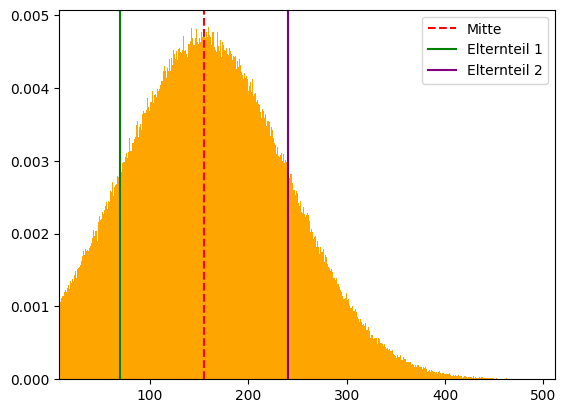
\includegraphics[width=1\linewidth]{rekombination.png}
	\caption{Normalverteilung bei der Rekombination für Batch-Größe}
	\label{fig:enter-label}
\end{figure}

\subsection{Selektion}
Die Selektion reduziert die Population nach der gewählten Strategie. So wird Platz für besser angepasste Individuen. Um bereits gefundene lokale Optimas nicht zu verlieren, werden pro Generation jeweils zwei Elitisten bestimmt, diese werden unverändert in die nächste Generation übernommen. Zusätzlich findet eine Turnierselektion zwischen zwei Chromosomen statt. Die Gewinner kommen in die nächste Generation, ein erneutes Auswählen findet nicht statt. So können auch schlechtere Chromosomen in die nächste Generation kommen, sodass lokale Optimas besser umgangen werden können. Durch die Turnierselektion wird die Population um 50\% reduziert.

\subsection{Mutation}
Die Mutation wird nach der Rekombination für jedes Konfiguration durchgeführt, die kein Elitist ist. Sie sorgt dafür, dass sich schlechtere wie auch bessere Konfigurationen verbessern oder verschlechtern können und sorgt für eine Diversität in der Population. Im genetischen Algorithmus wird jedes Gen mit einer Wahrscheinlichkeit von 20\% komplett neu generiert. So wird die Exploration verstärkt. 
\section{Bemerkungen zum Ansatz}
Der hier gewählte Ansatz hat seine Tücken. So ist die Wahl der Standardabweichung bei der Rekombination sehr wichtig, um eine Balance zwischen Exploration und Exploitation zu finden. In der Rekombination wird eher Wert auf die Exploitation gesetzt, während in der Mutation der Fokus auf die Exploration des Suchraums gesetzt wird. 